%% packages
\documentclass{article}
\usepackage[a4paper, left=2.0cm, right=2.0cm, top=3.5cm]{geometry}
\usepackage[ngerman]{babel}
\usepackage{graphicx}
\usepackage{multicol}
\usepackage{amssymb}
\usepackage{titlesec}
\usepackage{wrapfig}
\usepackage{blindtext}
\usepackage{lipsum}
\usepackage{caption}
\usepackage{listings}
\usepackage{fancyhdr}
\usepackage{nopageno}
\usepackage{authblk}
\usepackage{amsmath} % tons of math stuff
\usepackage{mathtools} % e.g. alignment within matrix
%\usepackage{bm} % provides shorthand for bold in math mode
\usepackage{dsfont} % \mathds makes double stroke digits
\usepackage{esdiff} % provides \diff
%\usepackage[ISO]{diffcoeff}
\usepackage{xcolor}
\usepackage{csquotes} % e.g. provides \enquote
\usepackage{siunitx} % units
\usepackage{xcolor} % colored text
%\fancyhf[]{}


%% custom stuff
% own units
\DeclareSIUnit \VSS {\ensuremath{V_\mathrm{SS}}}
\DeclareSIUnit \VS {\ensuremath{V_\mathrm{S}}}
\DeclareSIUnit \Veff {\ensuremath{V_\mathrm{eff}}}
\DeclareSIUnit \Vpp {\ensuremath{V_\mathrm{pp}}}
\DeclareSIUnit \Vp {\ensuremath{V_\mathrm{p}}}
\DeclareSIUnit \VRMS {\ensuremath{V_\mathrm{RMS}}}
\DeclareSIUnit \ASS {\ensuremath{A_\mathrm{SS}}}
\DeclareSIUnit \AS {\ensuremath{A_\mathrm{S}}}
\DeclareSIUnit \Aeff {\ensuremath{A_\mathrm{eff}}}
\DeclareSIUnit \App {\ensuremath{A_\mathrm{pp}}}
\DeclareSIUnit \Ap {\ensuremath{A_\mathrm{p}}}
\DeclareSIUnit \ARMS {\ensuremath{A_\mathrm{RMS}}}

% change subsection numbering to capital letters
\newcommand{\subsectionAlph}{ \renewcommand{\thesubsection}{\arabic{section}.\Alph{subsection}} }
% change subsection numbering to lowercase letters
\newcommand{\subsectionalph}{ \renewcommand{\thesubsection}{\arabic{section}.\alph{subsection}} }
% own fig. that works with multicols
\newenvironment{Figure}
  {\par\medskip\noindent\minipage{\linewidth}}
  {\endminipage\par\medskip}
\newcommand*{\inputPath}{./plot} % prepend this command to the argument of all input commands
\graphicspath{ {./figure/} }


% own commands
% \newcommand{\rarr}{$\to\,$} %A$\,\to\,$B
\newcommand{\defc}{black}
\newcommand{\colorT}[2][blue]{\color{#1}{#2}\color{\defc}}
\newcommand{\redq}{\color{red}(?)\color{\defc}}
\newcommand{\question}[1]{\colorT[purple]{\textbf{(#1)}}}
\newcommand{\todo}[1]{\colorT[red]{\textbf{(#1)}}}
\newcommand{\mr}{\mathrm}

%% preparation
\begin{titlepage}
    \title{Elektronikpraktikum: Versuch 2 \\Diodenkennlinien}
    \author[1]{Marc Hauer\thanks{s??mhaue@uni-bonn.de}}
    \author[1]{Michael Vogt\thanks{s65mvogt@uni-bonn.de}}
    \affil[1]{Uni Bonn}
    %\date{\today}
\end{titlepage}


%% document
\begin{document}

\pagenumbering{gobble}
\maketitle
\tableofcontents
\newpage
\pagenumbering{arabic}

\pagestyle{fancy}
\fancyhead[R]{\thepage}
\fancyhead[L]{\leftmark}


Es sollen Kennlinien von herkömmlichen und Zener-Dioden untersucht werden.
Außerdem werden Gleichrichtungsschaltungen mithilfe von Dioden, ggf. mit zusätzlicher Stabilisierung, gebaut.

\section{Theorie}
\todo{Physik hinter Dioden genauer erklären?}
Dioden bestehen aus einem n- und einem p-Dotierten Halbleiter in Kontakt miteinander. Am pn-Übergang kommt es zu Rekombination
der freien Elektronen (vom n-Typ) mit den Löchern (vom p-Typ), wodurch eine \textit{Verarmungszone}
mit Raumladungen und keinen freien Ladungsträgern entsteht. Dort gibt es ein Elektrisches Feld, welches vom n- zum p-Bereich zeigt.
Eine äußere Spannung mit der gleichen Orientierung vergrößert nur die Raumladungszone und es fließt kein Strom.
Zeigt die Spannung aber in die entgegengesetzte Richtung, kann die Raumladung aufgehoben werden und Strom fließen.
da zunächst das E-Feld in der Raumladungszone überwunden werden muss, gibt es eine \textit{Schwellspannung},
die überschritten werden muss, damit Strom in Durchlassrichtung fließt. In Sperrichtun

Wird eine Spannung in Sperrrichtung angelegt, fließt fast kein Strom, solange die Durchbruchspannung ($100-\SI{1000}{\V}$)
nicht überschritten wird. Wird sie überschritten, fließt ein hoher Strom und die Diode (außer bei Zenerdioden) wird i.d.R. zerstört.
% In Durchlassrichtung fließt Strom bei Überschreiten der \textit{Schwellspannung},
% welche deutlich niedriger als die Durchbruchspannung ist.
Das Verhalten des Stroms in Abhängigkeit der Spannung wird als
\textit{Kennlinie} der Diode bezeichnet. Im Gegensatz zu Widerständen haben Dioden nichtlineare Kennlinien.

Das Verhalten von Dioden kann u.A. genutzt werden, um Gleichrichtungsschaltungen zu bauen (Abb. \ref{fig:gleichrichter}).
Ein Einweggleichrichter wird mit einer einzigen Diode in Reihenschaltung zur Wechselspannungsquelle erreicht.
Als Zweiweggleichrichter fungiert die \textit{Graetzschaltung} mit vier Dioden. 

\begin{figure}[h]
  \centering
  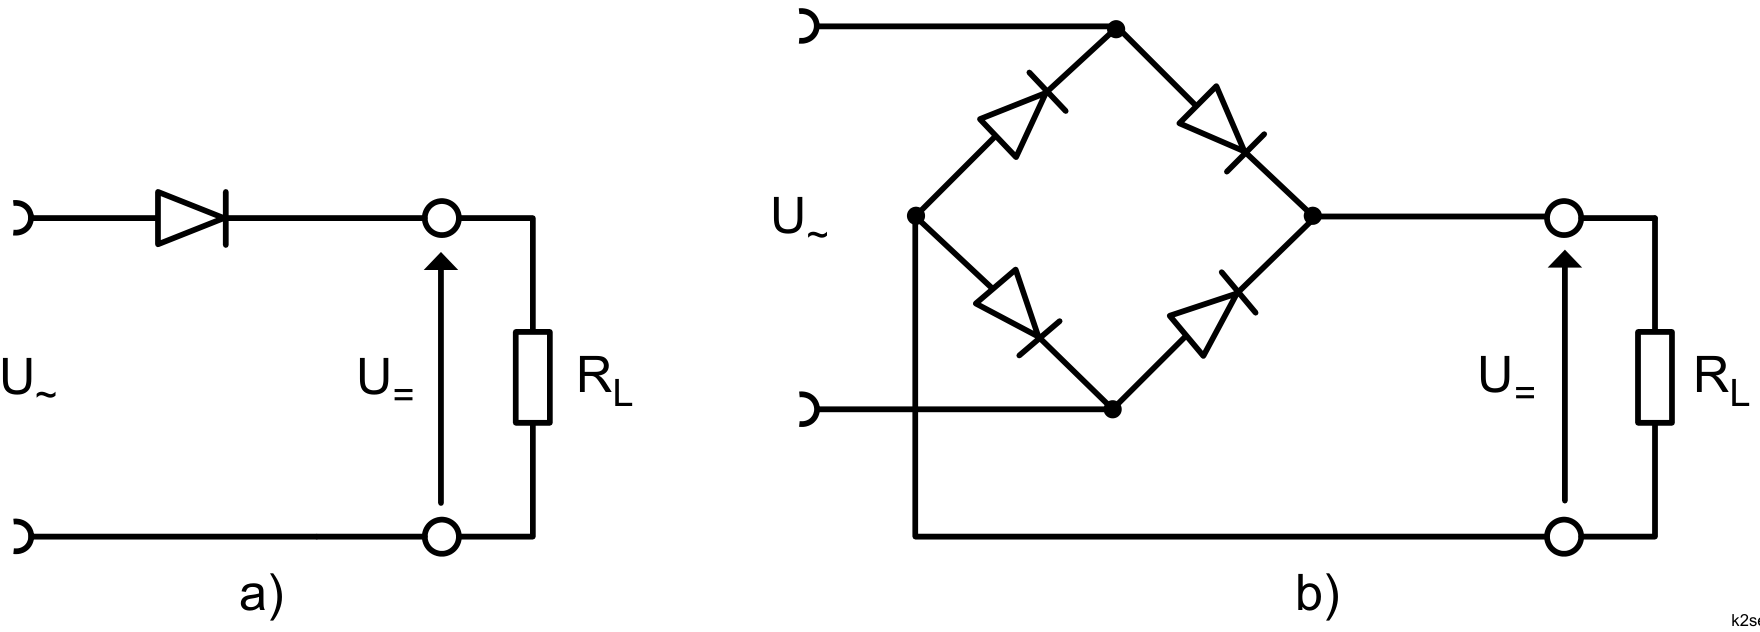
\includegraphics[width=0.4\textwidth]{gleichrichter}
  \caption{a) Einweggleichrichter, b) Zweiweggleichrichter}
  \label{fig:gleichrichter}
\end{figure}

Beide dieser Gleichrichtungsschaltungen produzieren eine Spannung mit konstantem Vorzeichen,
aber trotzdem starken periodischen Fluktuationen (\enquote{Brummen}). Zur Stabilisierung kann
ein Kondensator, oder eine Zenerdiode, zur Last parallel geschaltet werden. \question{wie funktioniert das mit der Zenerdiode?}
Der Kondensator wird bis zum Erreichen des Spannungsmaximums geladen. Wenn die äußere Spannung wieder fällt,
Liefert der Kondensator stattdessen die Spannung. Je mehr Strom fließt, desto schneller entlädt sich der Kondensator
wieder und je schneller fällt diese Spannung. Kondensatoren mit höherer Kapazität bauen mehr Ladung auf und können
die Spannung daher länger halten. 



\section{Voraufgaben}
\begingroup \subsectionAlph

\subsection{}
Die Dicke der Grenzschicht eines p-n-Halbleiters wird bestimmt durch das Material, den Grad der Dotierung
(d.h. die Konzentration von Donatoren und Akzeptoren) und die angelegte Spannung.

\subsection{}
Durch die Sperrschicht verhält sich eine Diode wie ein Plattenkondensator,
hat also eine Kapazität $C = \epsilon_0 \epsilon_r \frac{A}{d}$, wobei $d$ die Dicke der Sperrschicht ist.
Die Sperrschicht wird mit höherer angelegter Spannung in Sperrichtung breiter,
die Kapazität sinkt also mit steigender Spannung.

\subsection{}
{\centering 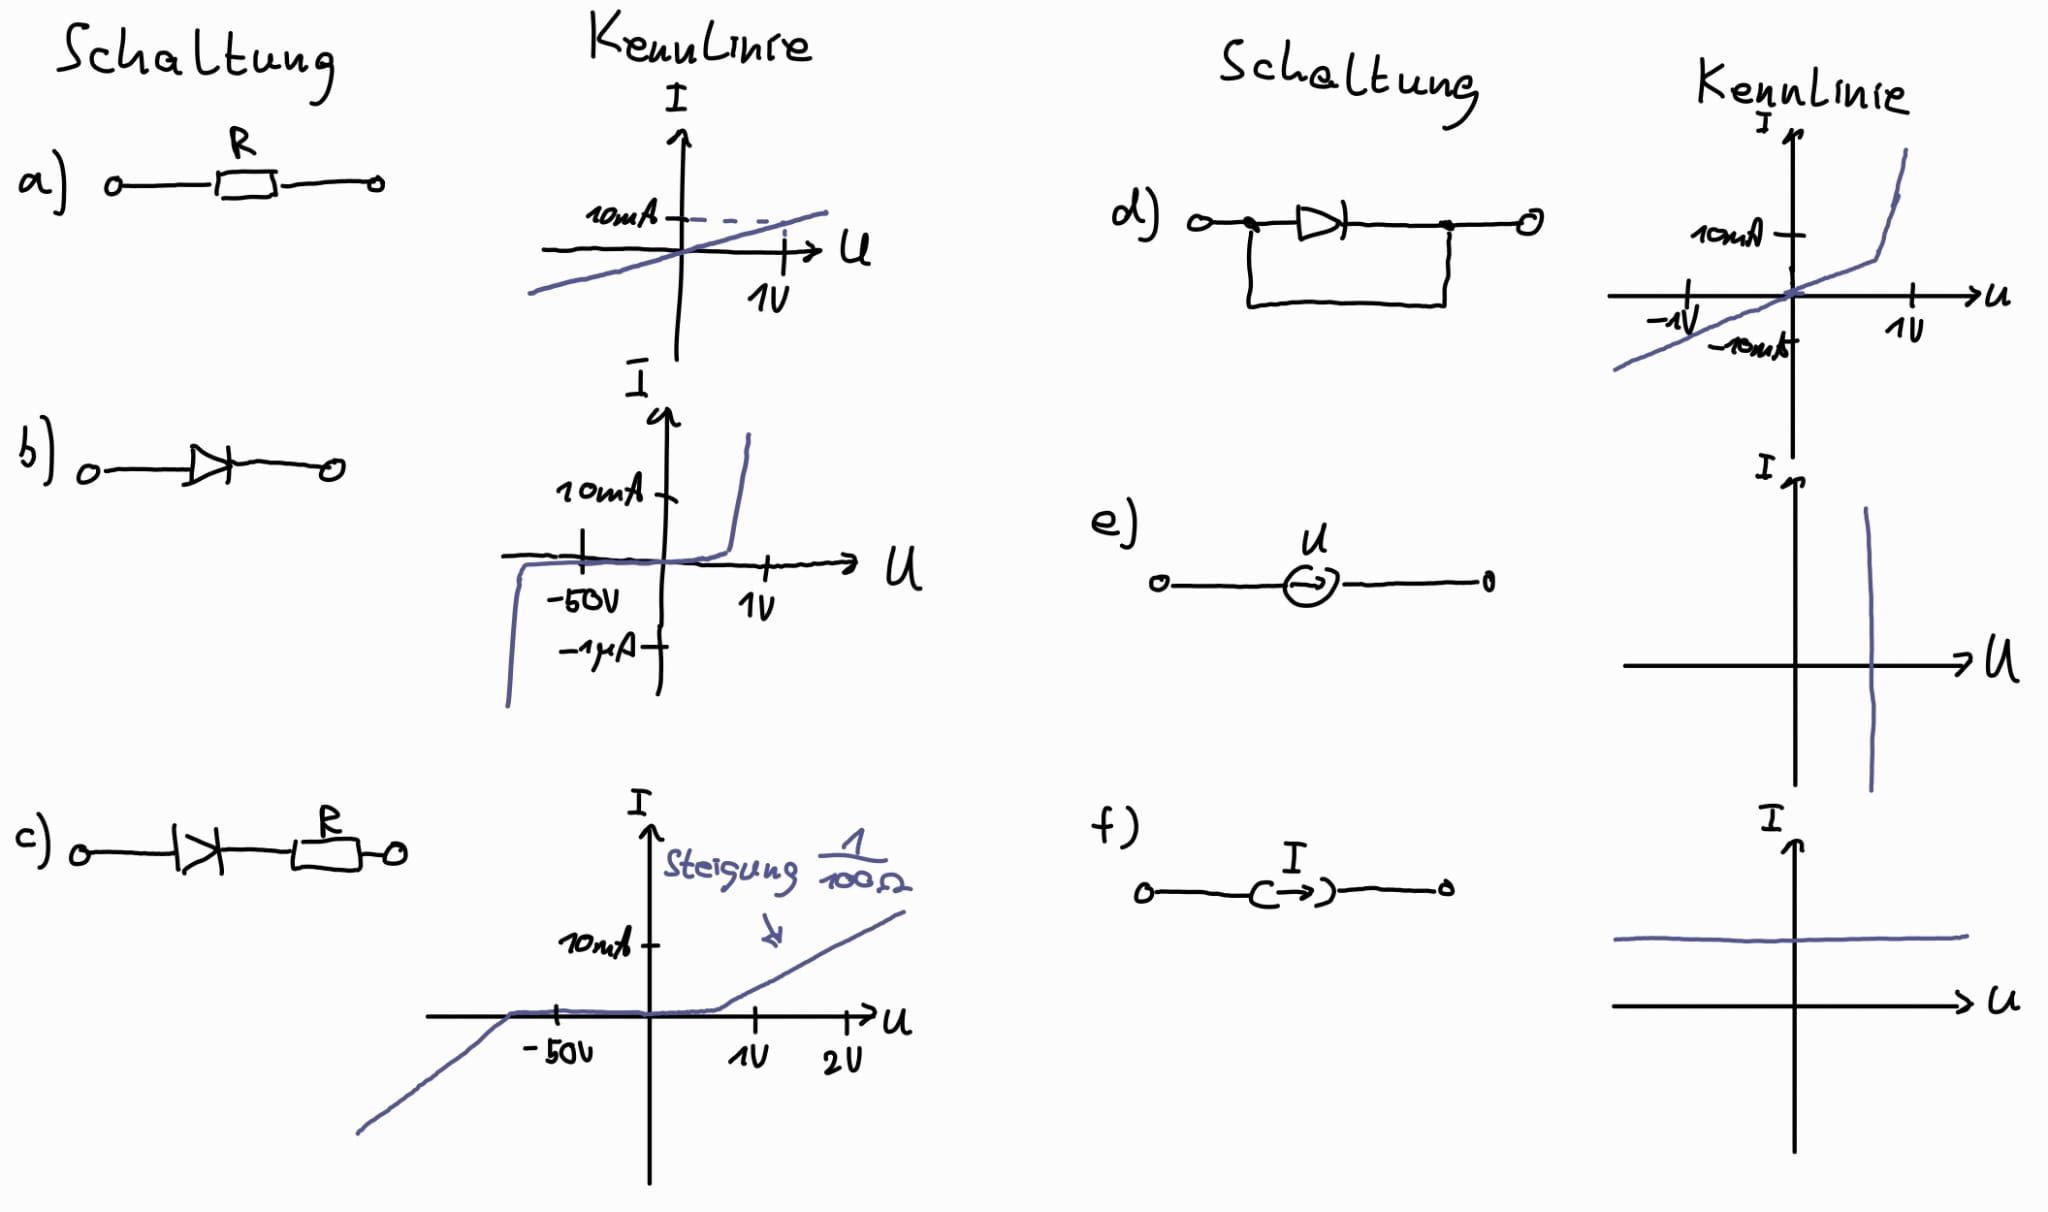
\includegraphics[width=0.6\textwidth]{aufgabeC}}
% \caption{a) Einweggleichrichter, b) Zweiweggleichrichter}
% \label{fig:aufgabeC}

\subsection{}
{\centering 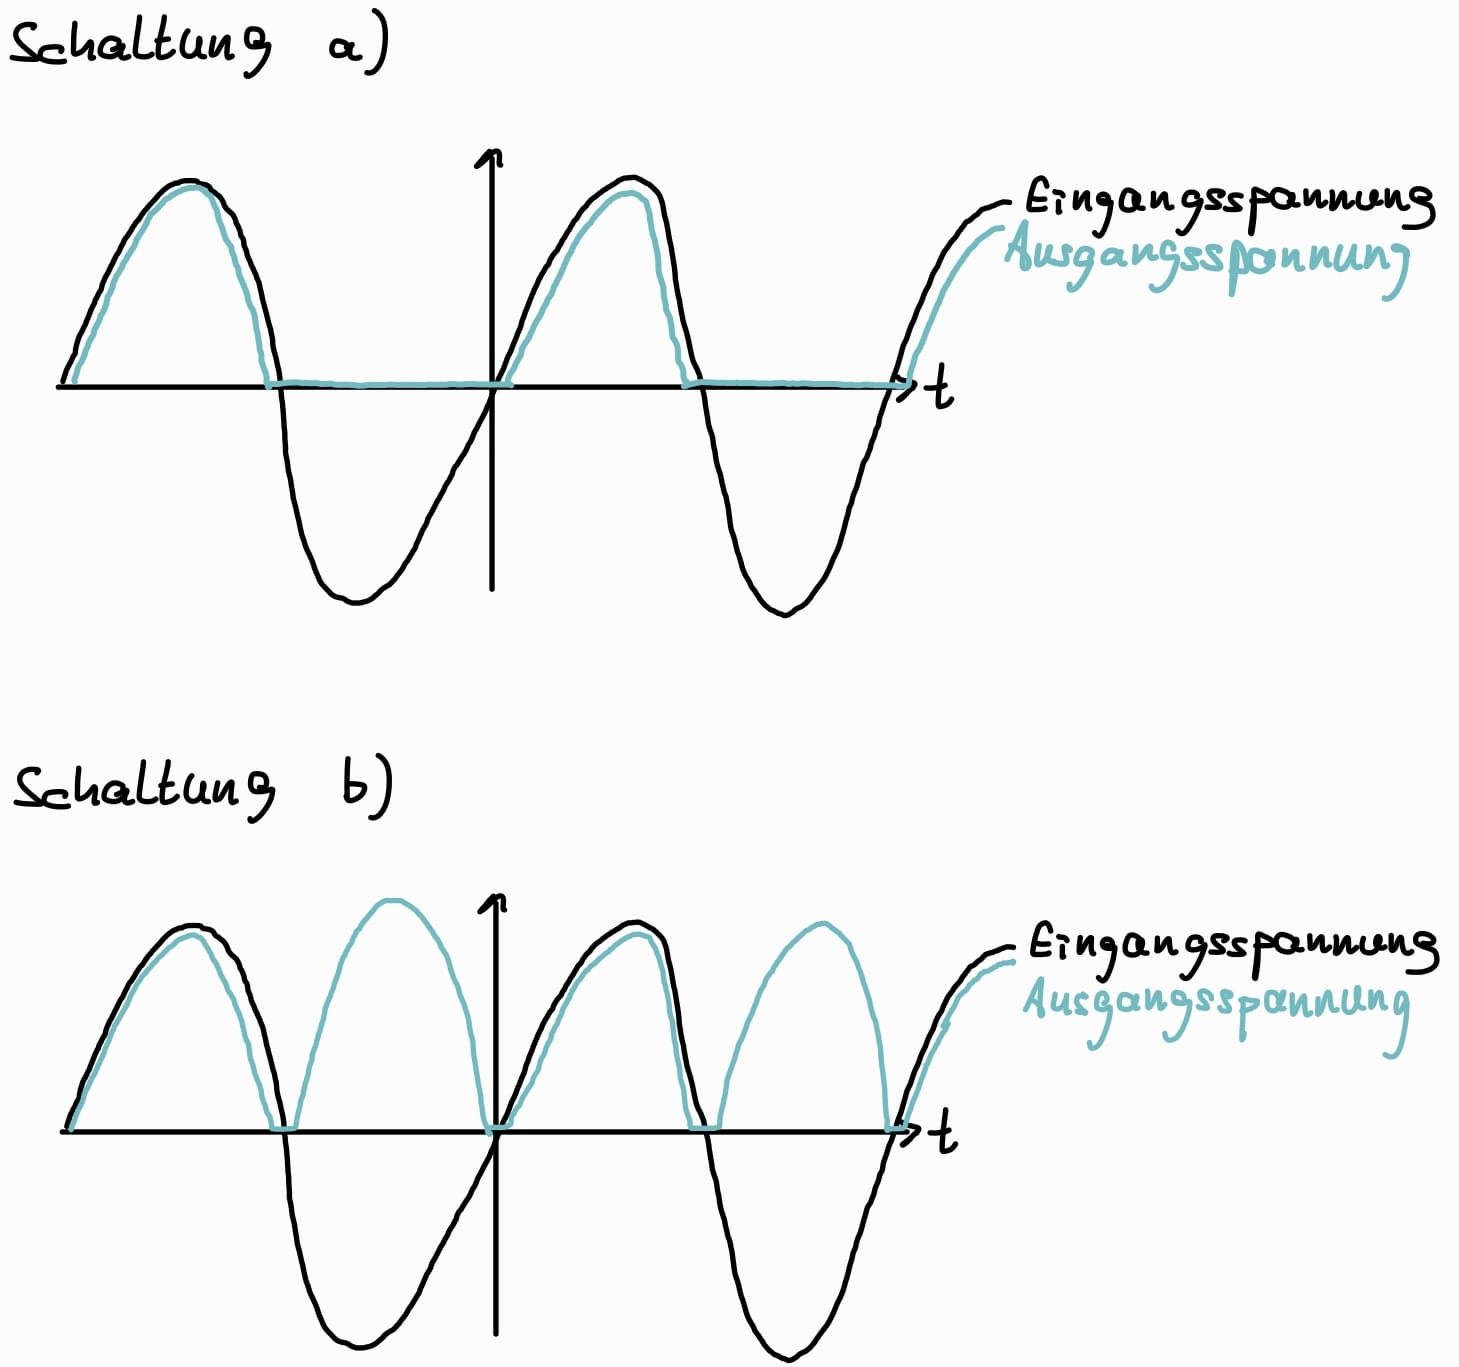
\includegraphics[width=0.4\textwidth]{aufgabeD}}
% \label{fig:aufgabeD}

\subsection{}
Je größer die Kapazität des Kondensators, desto mehr Ladung speichert er (bei gleicher Spannung)
und desto kleiner ist der Anteil der Gesamtladung, den er pro Sekunde durch den fließenden Strom verliert.
Um die Welligkeit der Spannung zu minimieren, muss also ein Kondensator möglichst großer Kapazität gewählt werden,
da die Spannung dann langsamer sinkt.

\subsection{}
Zur Messung der Spannung an und des Stroms durch die Diode muss überlegt werden, welche Größe präziser gemessen werden soll.
Da in Durchlassrichtung bei relativ niedriger Spannung hohe Ströme fließen, sollte hier Spannungsrichtig gemessen werden.
In Sperrichtung hingegen sollte selbst bei hohen Spannungen fast kein Strom fließen, weshalb wir stromrichtig messen sollten.

\subsection{}
Eine Zum Strom proportionale Spannung kann nach dem Ohm'schen Gesetz durch Reihenschaltung eines Widerstands erhalten werden.

\subsection{}
\question{Ich versteh gar nix}
Die Kapazität darf maximal so hoch sein, dass der Maximalstrom $I_\mr{max} = \SI{1000}{\mA}$ nicht erreicht wird. Also
\begin{equation}
  C = \frac{Q}{\Delta U} = \frac{I_\mr{max} \Delta t}{\Delta U} = \frac{\SI{1}{\A} \cdot \SI{1e-4}{\s}}{\SI{1}{\V}} = \SI{100}{\pF}
\end{equation}

\subsection{}
{\centering 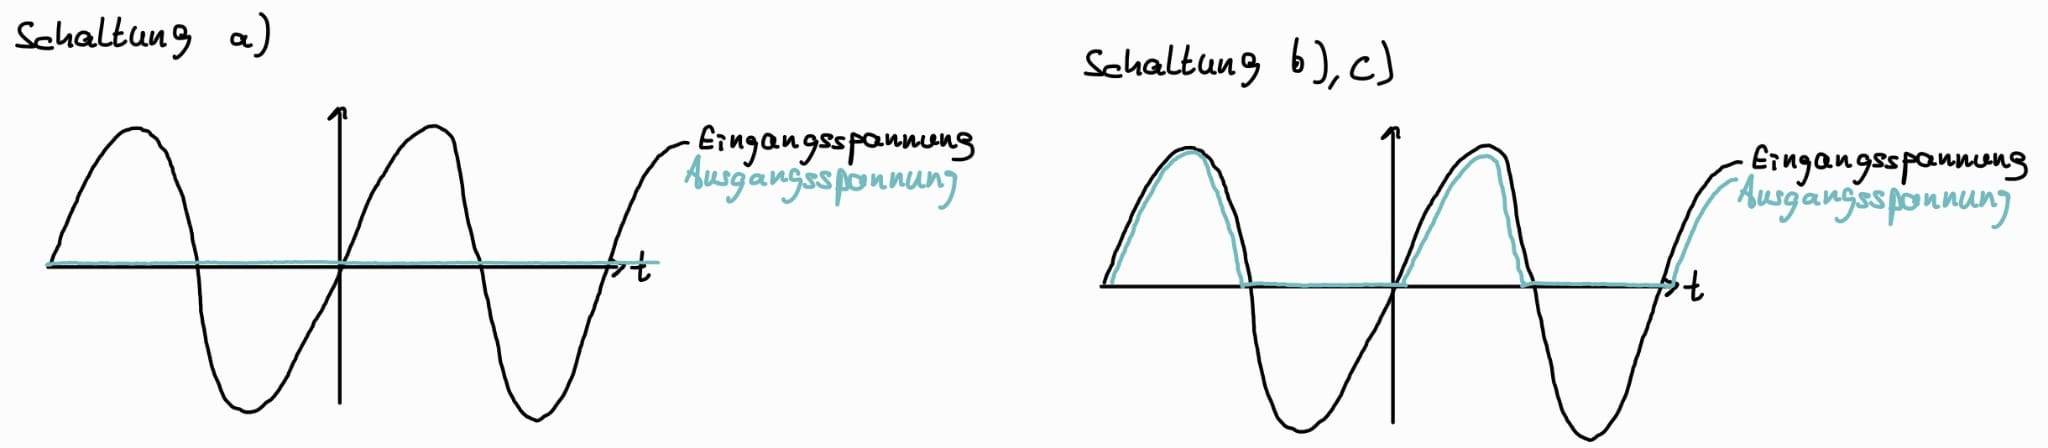
\includegraphics[width=0.9\textwidth]{aufgabeI}}

\subsection{}
{\centering 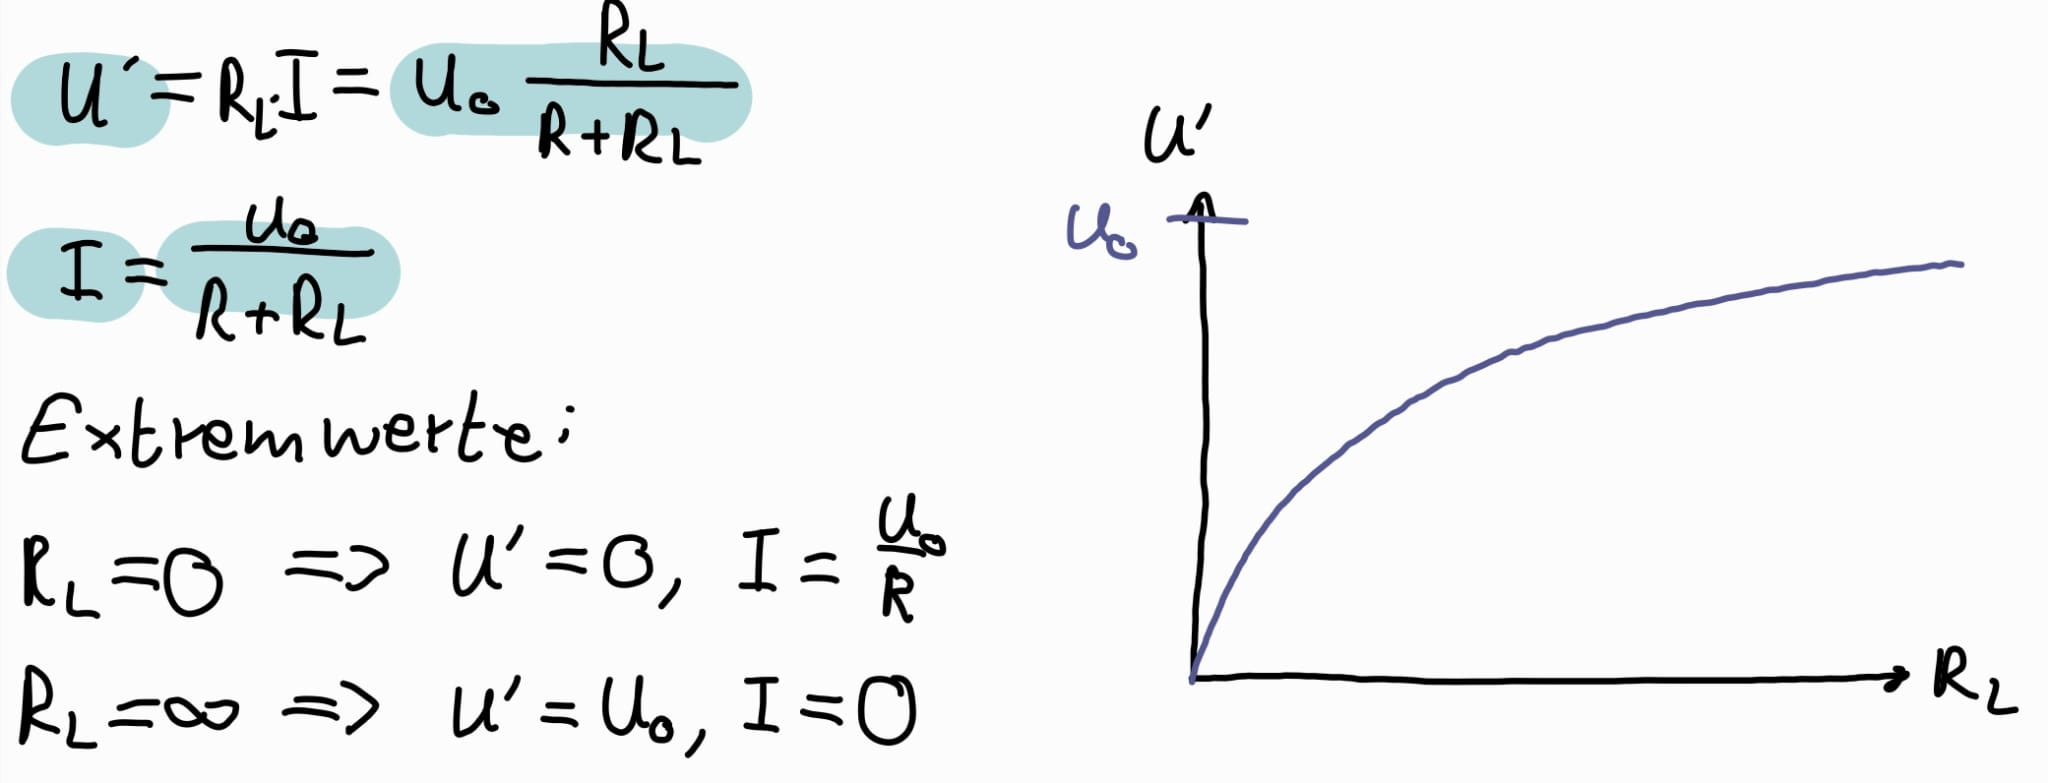
\includegraphics[width=0.4\textwidth]{aufgabeJ}}

\subsection{}
\todo{Muss noch gemacht werden!}

\endgroup

\end{document}
